\chapter{Process}
% \setcounter{section}{0}
\label{chapter:process}


The guidebook proposes a straightforward four-step assessment workflow:

\begin{center}
  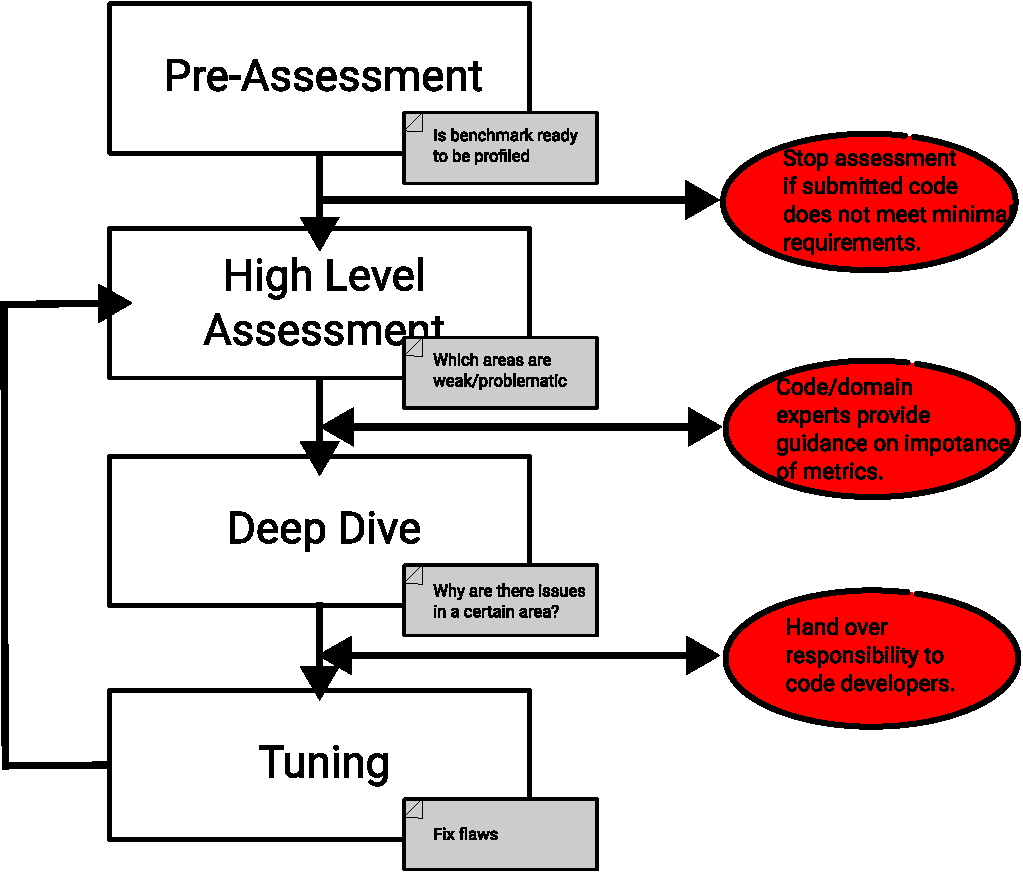
\includegraphics[width=0.7\textwidth]{process/workflow.pdf}
\end{center}


\begin{enumerate}
  \item 
    The \emph{pre-assessment} (Chapter~\ref{chapter:preparation}) determines whether the code is ready to be assessed. 
    It verifies that the code installs without expert knowledge, exposes the required configuration knobs, passes basic sanity checks, and meets minimum requirements.
    It validates that it offers a well-suited benchmark. 
    This phase is carried out by the benchmarking team, but it is the code authors' responsibility to ensure all requirements are met. 
    If they are not, the assessment terminates: 
    an assessment team cannot work productively continue.
  \item 
    The \emph{high-level assessment} (Chapter~\ref{chapter:high-level}) examines five areas of interest independently, identifying where the code performs well and where problems arise. 
    Studying the five areas separately has drawbacks, but sharpens the focus of subsequent steps. 
    This phase is conducted by the assessment team without involvement from the code developers.
    However, its findings must be interpreted and weighted collaboratively with the developers, who also indicate whether further in-depth analysis is warranted.  
  \item 
    Once areas of concern are identified, the \emph{in-depth assessment} (chapters from Part~\ref{part:performance-assessment}) drills into specific weaknesses to diagnose why the code underperforms. 
    This phase is again conducted independently by the assessment team, informed by the feedback gathered in the previous step.
  \item
    The findings feed into \emph{code tuning}. 
    This falls within the broader scope of performance engineering rather than the core assessment, and should ultimately trigger a re-assessment of the codebase.
\end{enumerate}


\section{Goals}


The phased process is built around three core principles.
They shape the workflow above.


\begin{itemize}
  \item {\bf Objectivity}. 
    The assessment must be objective and free of bias. 
    This requires a strict separation between the roles of assessor and code owner (developer), even in cases where the same person occupies both roles.
  \item {\bf Autonomy}. 
    Assessments can be conducted in close collaboration with developers or kept entirely separate. 
    The POP methodology, for example, requires strong involvement from code owners.
    By contrast, EuroHPC technical assessments for resource allocation aim to minimise such involvement---the assessor should require no knowledge of the codebase. 
    The present methodology follows the latter tradition.
  \item {\bf Responsibility}. 
    The process assigns clear ownership over who delivers what, and when. 
    Defined check-in points require developers to deliver specific inputs, while deliberately excluding them from other phases---keeping the workflow productive for the assessment team and assigning the ownership of the analysis to the assessment experts.
\end{itemize}

\noindent
Further to that, we introduce a two additional conventions:

\begin{itemize}
  \item 
    {\bf Specificity}. The assessments are machine-specific, benchmark-specific and configuration-specific.
    They make no attempt to generalise for the code over multiple machines, for different benchmark settings, or even only configurations of certain (hyper-)parameters such as GPU warp sizes, cores per rank, or MPI buffer settings.
    This means that all statements refer to the specific test setup.
    They can make statements along the lines ``this code scales poorly for this particular configuration of cores per rank'', but it is not possible to derive further, deeper insight;
    although it is obviously possible to compare the same assessments for the same code for multiple machines with each other, or to derive improved system setups from the analysis.
  \item
    {\bf Hypothesis-driven}. The assessment follows certain universal guidelines, but the subsequent deep dives, i.e.~the actual performance analysis is strictly hypothesis-driven.
    Once we start to explain why a code behaves in a certain way (cf.~Section~\ref{section:terminology:what-we-do}), we start with a hypothesis, evaluate this hypothesis and then either confirm it and dive deeper or discard it and study the next hypothesis.
\end{itemize}


\section{Criticism}

\begin{assessmentcrime}
 The roles of performance analyst and performance engineer are not carefully separated.
\end{assessmentcrime}


There are at least two alternative schools of thought when it comes to performance analysis.
The the first school emphasises that constructive performance improvements can only result from a dialogue between performance expert and code owner.
They point out that performance assessment or analysis is difficult if not impossible if there's no context on the code's structure, algorithms, data sets, objectives, and so forth.

Our strategy appreciates the need for a feedback cycle, but is anxious of the bias introduced by a very close collaboration.
We have seen multiple cases, where code owners almost expected the performance analysis to ``tell me what I want to hear'':
they did steer the analysis down a certain route, and expected instructions how to improve the code parts they had been interested anyway rather than an objective assessment of the overall ``product''.

This is the reason why our document advocates for a strict separation of the role of the assessor and the code expert.
That does not mean that the assessor may not know anything of the code and should not speak to the code owner.
It also does not mean that these two roles always have to be separate people. 
One person can switch hats.
It however does ask for a strict separation and the attempt to avoid that any code knowledge influences the assessment.
Again, the analogy to a GP helps:
A good GP will always ask the patient where it hurts, but they will be very critical when they are told about self-diagonses (guided by Google).

A second school of thought is strongly metrics- or data-driven.
Here, the idea is that it is key to gather as many metrics as possible initially and to distill hypotheses and eventually insights from these data.
The approach is popular with tool developers.

Our document advocates for a hypothesis-driven workflow, where a hypotheses or metric of interest determine what data is of interest.
Once this is clear, we suggest that assessors pick a tool to gather these data---often a different tool per purpose.
Both approaches, hypothesis- and data-driven come along with pros and cons. 
In practice, many performance analysis will employ a hybrid.
However, we favour the workflow and sequence of hypotheses guiding what data is gathered in this write-up.


\section{Shortcomings}


Like any process, the current approach carries trade-offs.

First, the strict separation of roles and the emphasis on autonomy demand a certain level of code maturity: 
the code must be usable by a non-expert with little to no prior knowledge of the codebase or domain. 
In particular in agile projects in scientific computing, where the user base is often very small and highly specialised, these risks are particularly pronounced. 
While the process excludes developers from the majority of the assessment, it requires strong commitment from the code owners to deliver a ready-to-use benchmark in the first place.

Second, the reliance on reports as the primary output also creates a risk of conflict, as developers may dispute findings and bristle at how they are presented.
This is particularly important in scientific code development projects, where code authors develop a strong emotional attachment to code, since they build their career on it.
A successful delivery of (multiple) code assessments requires a constructive collaboration.
The fact that the process tries to be as objective and therefore somtimes might yield brutal insights or performance statements, challenges constructive collaboration.
This has to be taken into account (and moderated) by the involved senior managers. 

Third, the attempt to isolate performance flaws and metrics bears risk to separate flaws that are strongly correlated.
For example, poor core utilisation on some cores might lead to a situation where the overall load balancing appears to be weak.
The assessment handles these metrics independently and hence runs risk to report balancing issues rather than the cause of the problem.
This is an example, where domain and code expertise can help, but it remains a fundamental drawback baked into the process itself.

Finally, both the role separation and the exclusion of optimisation work create a risk of losing expert knowledge embedded in the code or domain. 
This tension is addressed in the wrap-up discussion (Section~\ref{section:high-level:wrap-up}), which acknowledges that independent assessments can struggle to connect findings to scientific requirements. 
Prioritising steps, metrics, and studies nevertheless remains difficult. 
The present approach always risks trading independence and objectivity for deeper insight.


 